% Provenance (never printed): see sources/outline_sources.md and sources/book1/BRIEFS.md (g3/01).
\chapter{Typing with Ten Fingers}\label{ch:g3:typing-with-ten-fingers}

Noor is typing a story for school. She uses two fingers, one on each hand. Her
eyes go down to the keys to find a letter, up to the screen to check it, down
again for the next letter. Her big sister Lina, at the other end of the table,
types with all ten fingers. Her eyes never leave the screen, and she types
twice as fast as Noor, with fewer mistakes. Lina is not magic: she learned a
technique, and anybody can learn it.

\begin{recall}
\key{Shift} is held down while another key is pressed, to type a capital or
the sign drawn at the top of a key. Sit with your back against the chair, your
feet flat and your forearms level (\cref{ch:g2:keyboard-and-mouse}).
\end{recall}

\section{The home row}

\begin{definition}[Touch typing]\label{def:g3:typing-with-ten-fingers:touch-typing}
\emph{Touch typing}\index{touch typing} is typing with all ten fingers
without looking at the keys: each finger always strikes the same keys and
finds them by touch.
\end{definition}

For \omterm{def:g3:typing-with-ten-fingers:touch-typing}{touch typing}, the hands always start from the same place and come back to
it after each key.

\begin{definition}[Home row]\label{def:g3:typing-with-ten-fingers:home-row}
The \emph{home row}\index{home row} is the middle row of letter keys, where
the fingers rest between two keys: on a QWERTY keyboard, the left hand rests
on A S D F and the right hand on J K L and the key after L; the thumbs rest
on the space bar.
\end{definition}

% ledger: typ:bumps
How can the hands find the \omterm{def:g3:typing-with-ten-fingers:home-row}{home row} without looking? Feel the F and J keys:
on most keyboards, each carries a small bump. Put your index fingers on the two
bumps, and the other fingers fall into place beside them.

\begin{omfigure}
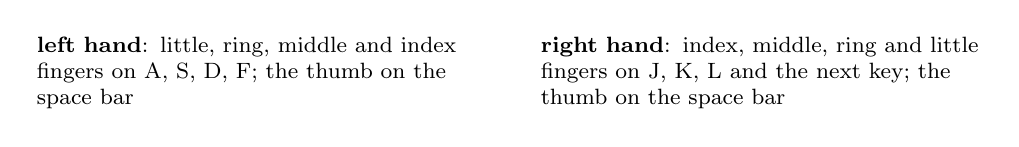
\begin{tikzpicture}[font=\footnotesize]
  \omkeyboardkeys[unit=0.82cm, home, highlight={AC01,AC02,AC03,AC04,AC07,AC08,AC09,AC10,SPCE}]{us}
  \node[anchor=north, align=left, text width=5.6cm] at (3.0,-4.3) {\textbf{left hand}: little, ring, middle and index fingers on A, S, D, F; the thumb on the space bar};
  \node[anchor=north, align=left, text width=5.6cm] at (9.4,-4.3) {\textbf{right hand}: index, middle, ring and little fingers on J, K, L and the next key; the thumb on the space bar};
\end{tikzpicture}

{\small The \omterm{def:g3:typing-with-ten-fingers:home-row}{home row}: eight fingers rest on the outlined keys, the thumbs on
the space bar. The F and J keys carry a small bump (the short line drawn on
them).}
\label{fig:g3:typing-with-ten-fingers:home-row}
\end{omfigure}

\begin{omfigure}
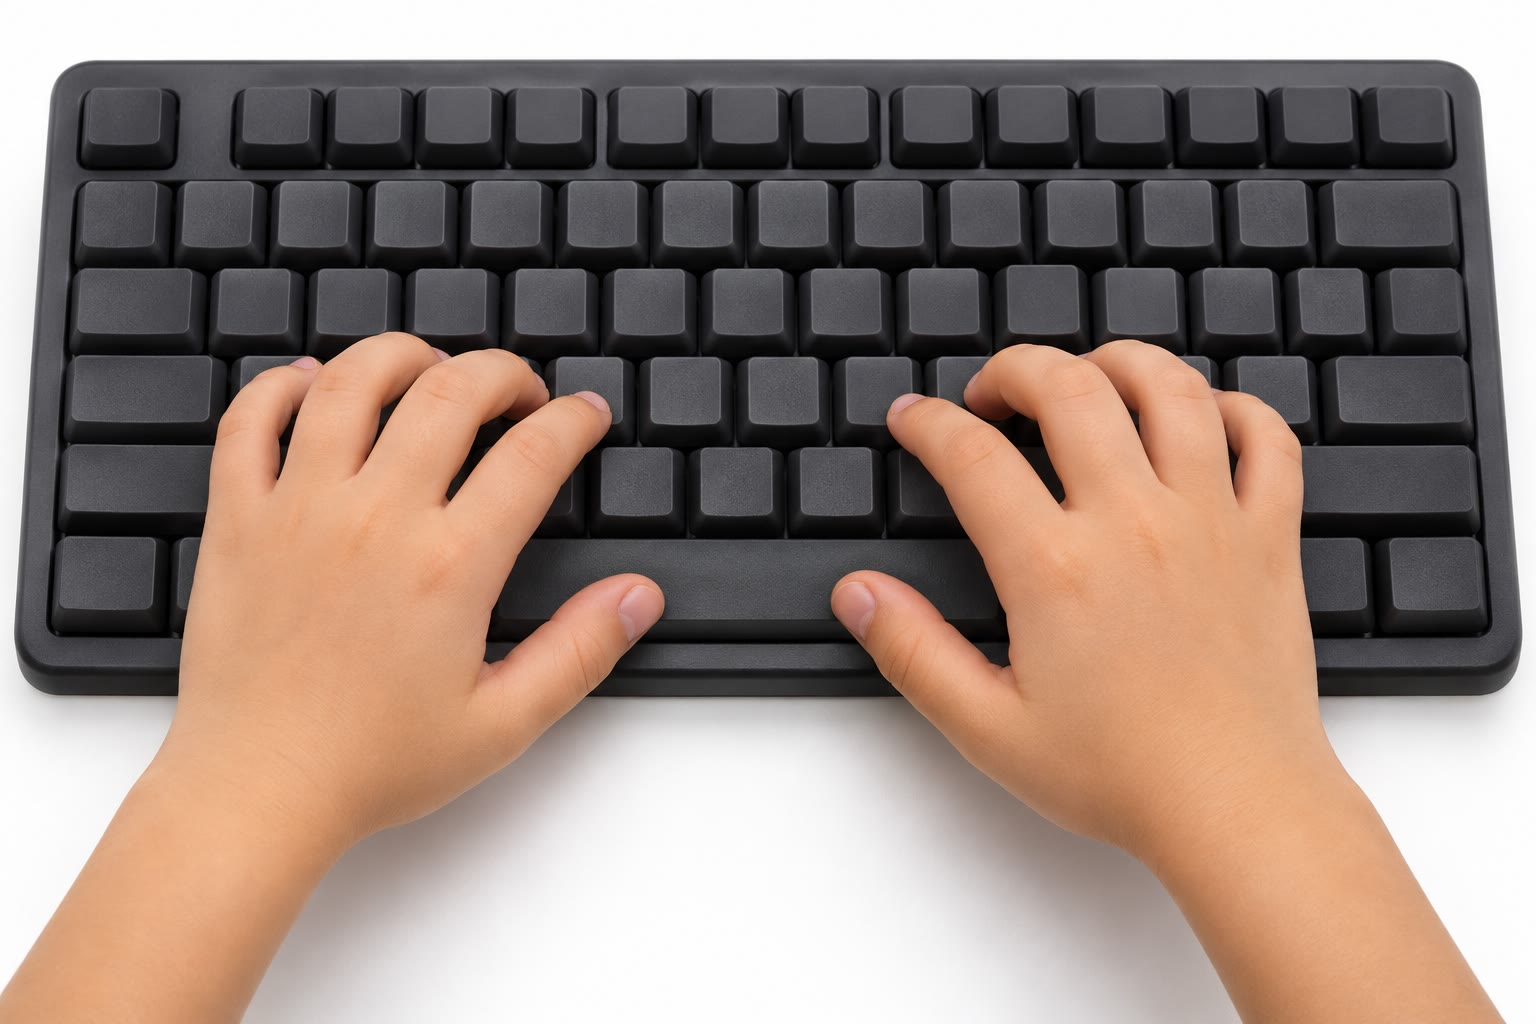
\includegraphics[width=0.58\linewidth]{images/book1/ai/g3-typing-with-ten-fingers-hands.jpg}

{\small Two hands resting on the \omterm{def:g3:typing-with-ten-fingers:home-row}{home row}: fingers curved, fingertips lightly
on the keys, thumbs over the space bar, wrists not touching the table.}
\end{omfigure}

\section{Which finger strikes which key}

Each finger owns a slanted column of keys: the key of the \omterm{def:g3:typing-with-ten-fingers:home-row}{home row} where it
rests, the key above it and a little to the left, and the key below it and a
little to the right. The index fingers are the strongest, so each owns two
columns: its own and the one next to it, towards the middle of the keyboard.
The little fingers own the keys at the edges: \key{Shift}, \key{Enter},
\key{Backspace}, \key{Tab}.

\begin{omfigure}
\begin{tikzpicture}[font=\footnotesize]
  \omkeyboardkeys[unit=0.82cm, fingers, home]{us}
  \foreach \c/\t [count=\k] in {omkbP/little fingers, omkbR/ring fingers, omkbM/middle fingers, omkbI/index fingers, omkbT/thumbs} {
    \fill[\c, draw=black!50] ({0.1+2.6*(\k-1)},-4.75) rectangle ++(0.4,0.3);
    \node[anchor=west, font=\scriptsize] at ({0.55+2.6*(\k-1)},-4.6) {\t};
  }
\end{tikzpicture}

{\small Each colour is one finger of each hand: the left hand types the left
part of the keyboard, the right hand the right part. Every key is typed by the
finger of its colour, which then comes back to the \omterm{def:g3:typing-with-ten-fingers:home-row}{home row}.}
\label{fig:g3:typing-with-ten-fingers:zones}
\end{omfigure}

\begin{method}[Striking a key]\label{met:g3:typing-with-ten-fingers:strike}
Start with all fingers on the \omterm{def:g3:typing-with-ten-fingers:home-row}{home row}. Move only the finger that owns the key,
strike the key lightly and quickly, and bring the finger straight back to its
home key. The other fingers stay where they are.
\end{method}

\begin{example}[Typing the word ``dog'']\label{ex:g3:typing-with-ten-fingers:dog}
D is on the \omterm{def:g3:typing-with-ten-fingers:home-row}{home row}, under the left middle finger: strike it. O is above L,
in the column of the right ring finger: the ring finger reaches up, strikes O
and comes back to L. G is next to F, in the second column of the left index
finger: the index finger slides one key to the right, strikes G and comes back
to F.
\end{example}

\section{Eyes on the screen}

At the start, the fingers do not know where the keys are, and it is tempting
to look down. But every time the eyes go down to the keys and back up to the
screen, we lose time and lose our place in the text. A touch typist looks at
the screen, or at the page being copied, and lets the fingers find the keys.
The eyes are then free to catch mistakes as soon as they appear.

Learning this takes some weeks of short daily practice. The appendix at the end
of this book, \emph{Typing drills}, gives lines to practise, one finger and one
row at a time.

\section{Capitals, digits and signs}

To type a capital, one little finger holds \key{Shift} while a finger of the
other hand strikes the letter: always the \key{Shift} of the \emph{other} hand.
For a capital J (right hand), the left little finger holds the left
\key{Shift}; for a capital A (left hand), the right little finger holds the
right \key{Shift}.

\begin{omfigure}
\begin{tikzpicture}[font=\footnotesize]
  \omkeyboardkeys[unit=0.82cm, highlight={LFSH,AC07,RTSH,AC01}]{us}
  \node[draw=ocRed!80!black, fill=white, rounded corners=2pt, inner sep=3pt] (cj) at (6.15,-5.0) {capital J: left \key{Shift} + J};
  \draw[ocRed!80!black, line width=0.9pt] (cj.north) -- (kb-LFSH.center) (cj.north) -- (kb-AC07.center);
  \fill[ocRed!80!black] (kb-LFSH.center) circle (1.5pt) (kb-AC07.center) circle (1.5pt);
  \node[draw=ocBlue!80!black, fill=white, rounded corners=2pt, inner sep=3pt] (ca) at (6.15,0.75) {capital A: right \key{Shift} + A};
  \draw[ocBlue!80!black, line width=0.9pt] (ca.south) -- (kb-RTSH.center) (ca.south) -- (kb-AC01.center);
  \fill[ocBlue!80!black] (kb-RTSH.center) circle (1.5pt) (kb-AC01.center) circle (1.5pt);
\end{tikzpicture}

{\small \key{Shift} is always held by the little finger of the other hand than
the one that strikes the letter.}
\label{fig:g3:typing-with-ten-fingers:shift}
\end{omfigure}

The digits are on the top row. Each finger reaches up two rows, from its home
key, to the digit of its column, and comes back. The signs (full stop, comma,
question mark) are typed by the finger that owns their key, with \key{Shift}
when the sign is drawn at the top of the key.

\begin{definition}[Keyboard layout]\label{def:g3:typing-with-ten-fingers:layout}
The \emph{keyboard layout}\index{keyboard layout} is the order in which the
letters, digits and signs are placed on the keys of a keyboard. A layout is
named after the first six letters of its top row of letters: QWERTY, AZERTY,
QWERTZ.
\end{definition}

% ledger: typ:layout-us, typ:layout-fr, typ:layout-de
Different countries use different layouts, so that the letters of their own
language are easy to reach. The technique is the same everywhere: the same
home position, the same fingers, the same columns. Only a few letters sit
under other fingers. On an AZERTY keyboard, the digits are typed with
\key{Shift}; without it, the top row types signs and accented letters.

\begin{omfigure}
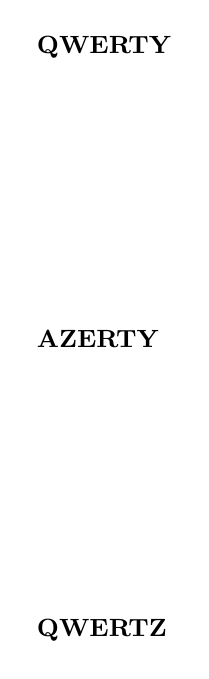
\begin{tikzpicture}[font=\footnotesize]
  \node[anchor=west, font=\small\bfseries] at (0,0.35) {QWERTY};
  \begin{scope}[shift={(0,0)}] \omkeyboardkeys[unit=0.62cm]{us} \end{scope}
  \node[anchor=west, font=\small\bfseries] at (0,-3.35) {AZERTY};
  \begin{scope}[shift={(0,-3.7)}] \omkeyboardkeys[unit=0.62cm, highlight={AD01,AD02,AC01,AC10,AB01}]{fr} \end{scope}
  \node[anchor=west, font=\small\bfseries] at (0,-7.05) {QWERTZ};
  \begin{scope}[shift={(0,-7.4)}] \omkeyboardkeys[unit=0.62cm, highlight={AD06,AB01}]{de} \end{scope}
\end{tikzpicture}

{\small Three \omterm{def:g3:typing-with-ten-fingers:layout}{keyboard layouts}. The outlined keys carry a letter that is
somewhere else on the QWERTY keyboard.}
\label{fig:g3:typing-with-ten-fingers:layouts}
\end{omfigure}

\begin{history}[Why the letters are in this order]
% ledger: typ:sholes-1874, typ:qwerty-origin
The order of the letters is older than \omterm{def:g1:what-is-a-computer:computer}{computers}. It comes from the typewriters
of Christopher Sholes, the first of which was offered for sale in 1874. The
letters of its top row already began Q, W, E, R, T, Y. One reason often given
is that letters often typed together were placed apart, so that the metal arms
that printed them would not get stuck together. People still discuss whether
that was the main reason. \omterm{def:g1:what-is-a-computer:computer}{Computers} kept the order that typists already knew.
\end{history}

\begin{omfigure}
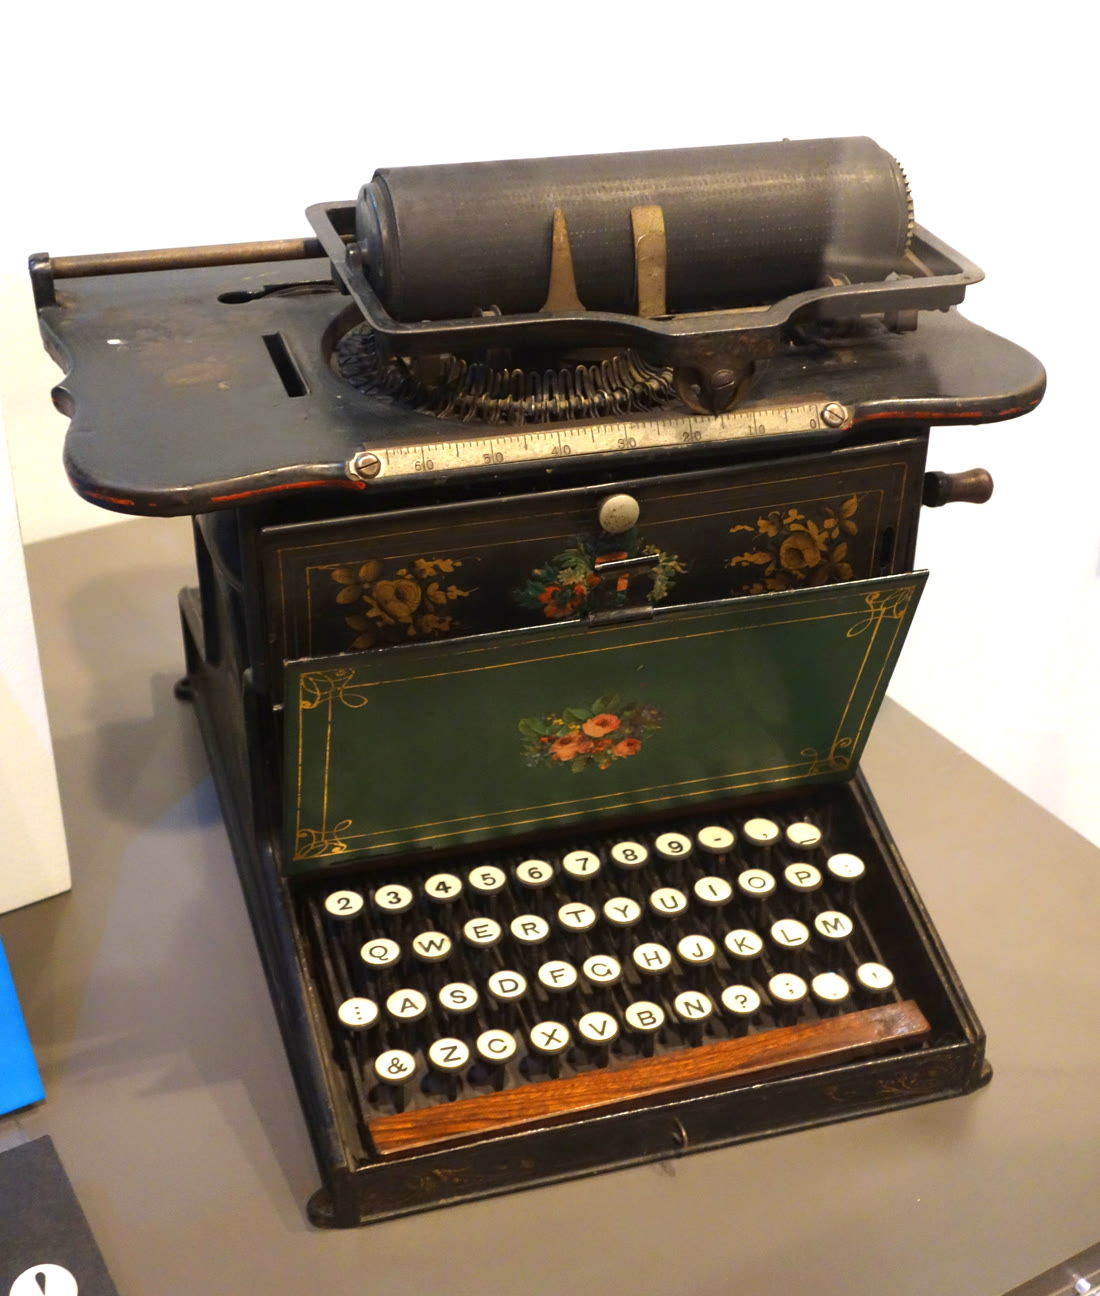
\includegraphics[width=0.42\linewidth]{images/book1/g3-sholes-glidden.jpg}

{\small A Sholes and Glidden typewriter, made by Remington in the 1870s. Look at
its second row of keys: Q W E R T Y U I O P. Wisconsin Historical Museum;
photograph by Daderot, CC0.}
\end{omfigure}

\section{Accuracy before speed}

When you learn, type slowly and without mistakes. Speed comes by itself with
practice; mistakes learned at the start are hard to unlearn. A mistake also
costs time: the letter must be rubbed out and typed again.

\begin{definition}[Words per minute]\label{def:g3:typing-with-ten-fingers:wpm}
The speed of typing is counted in \emph{words per minute}\index{words per
minute}: the number of characters typed, divided by five, divided by the
number of minutes. Every five characters, spaces and signs included, count as
one word.
\end{definition}

\begin{example}[A timed test]\label{ex:g3:typing-with-ten-fingers:test}
Noor copies a text for 2 minutes and types 200 characters. That makes
$200 \div 5 = 40$ words in 2 minutes, so $40 \div 2 = 20$ \omterm{def:g3:typing-with-ten-fingers:wpm}{words per minute}. A
month later she types 300 characters in 2 minutes: $300 \div 5 = 60$ words,
$60 \div 2 = 30$ \omterm{def:g3:typing-with-ten-fingers:wpm}{words per minute}.
\end{example}

\begin{remark}[Why five characters]\label{rem:g3:typing-with-ten-fingers:five}
Words have different lengths: ``a'' has one letter, ``\omterm{def:g1:what-is-a-computer:computer}{computer}'' has eight.
Counting characters and dividing by five makes the count fair for every text,
whatever the length of its words.
\end{remark}

\section{Exercises}

\begin{exercise}[$\star$]\label{exo:g3:typing-with-ten-fingers:1}
On a QWERTY keyboard, which finger types each of these letters: A, S, E, R,
T, J, O, P?
\end{exercise}

\begin{exercise}[$\star$]\label{exo:g3:typing-with-ten-fingers:2}
Which \key{Shift} do you hold for a capital A? For a capital L? With which
finger?
\end{exercise}

\begin{exercise}[$\star$]\label{exo:g3:typing-with-ten-fingers:3}
What are the small bumps on the F and J keys for?
\end{exercise}

\begin{exercise}[$\star$]\label{exo:g3:typing-with-ten-fingers:4}
Sami types 150 characters in 2 minutes. How many \omterm{def:g3:typing-with-ten-fingers:wpm}{words per minute} is that?
\end{exercise}

\begin{exercise}[$\star$]\label{exo:g3:typing-with-ten-fingers:5}
Lina types at 30 \omterm{def:g3:typing-with-ten-fingers:wpm}{words per minute} for 3 minutes. How many characters does she
type?
\end{exercise}

\begin{exercise}[$\star$]\label{exo:g3:typing-with-ten-fingers:6}
Give three habits that make typing slow.
\end{exercise}

\begin{exercise}[$\star$]\label{exo:g3:typing-with-ten-fingers:7}
Look at the drawing of the three layouts. Which letters are not in the same
place on a QWERTY and an AZERTY keyboard? On a QWERTY and a QWERTZ keyboard?
\end{exercise}

\begin{exercise}[$\star\star$]\label{exo:g3:typing-with-ten-fingers:8}
List the fingers that type the word ``home'' on a QWERTY keyboard, in order.
\end{exercise}

\begin{exercise}[$\star\star$]\label{exo:g3:typing-with-ten-fingers:9}
In one minute, Tom types 120 characters with 6 mistakes, and Mia types 100
characters with no mistake. Who practises in the better way? Why?
\end{exercise}

\begin{exercise}[$\star\star$]\label{exo:g3:typing-with-ten-fingers:10}
Leo practises typing 10 minutes a day. How many days does he need to practise
15 hours in all?
\end{exercise}

\begin{exercise}[$\star\star$]\label{exo:g3:typing-with-ten-fingers:11}
Why do the index fingers own two columns of keys each, and the little fingers
the keys at the edges?
\end{exercise}
